\chapter{The Lattice Boltzmann Algorithm}
\section{General Description}
As previously asserted, the heart of the Lattice-Boltzmann Algorithm lies on its discretization of the phase space\cite{franco} \cite{integerLatticeDynamics}. To discretize the phase space, one must first choose the region to simulate. In this work, we name the extremal values in the $w$ axis of the phase space $W_{min}$ and $W_{max}$. Then, one has to fix either the size of the grid or the size of the lattice. We named the size of the grid in the $w$ axis $N_w$ (i.e. $N_x$ or $N_{vz}$). The size of the lattice in the $w$ axis ($dw$) and the extremal values are related by:
% $$ dk = \frac{K_{max}-K_{min} }{N_k}  $$
\begin{equation}
dw = \frac{W_{max}-W_{min} }{N_w} 
\end{equation}

In this work we are going to use the density-velocity phase space. Now that we have properly defined the phase space grid, we can proceed to the initialization. For simplicity, we choose gaussian initial conditions given by:
\begin{equation}
\f[0]= A \exp{-\frac{\vb{r}^2}{\sigma_r^2} - \frac{\vb{v}^2}{\sigma_v^2}}
\end{equation}
Where $\f[0]$ is the initialization of the phase space, $A$ is an indirect measure of the total mass in the system, $\vb{r}$ is the vector = $(x,y,z)$, $\vb{v}$ is the vector = $(vx,vy,vz)$, and $\sigma_r$ and $\sigma_v$ are a measure of the width of the gaussian profile in the given axis. After initialization, the system evolves by classical mechanics and the modelling of the collisional step, which can be seen more easily in figure  \ref{flowchart}

\begin{figure}[H]
    \centering
    %\includegraphics[width=10cm,height =7cm]{Diapositiva1.jpg}
    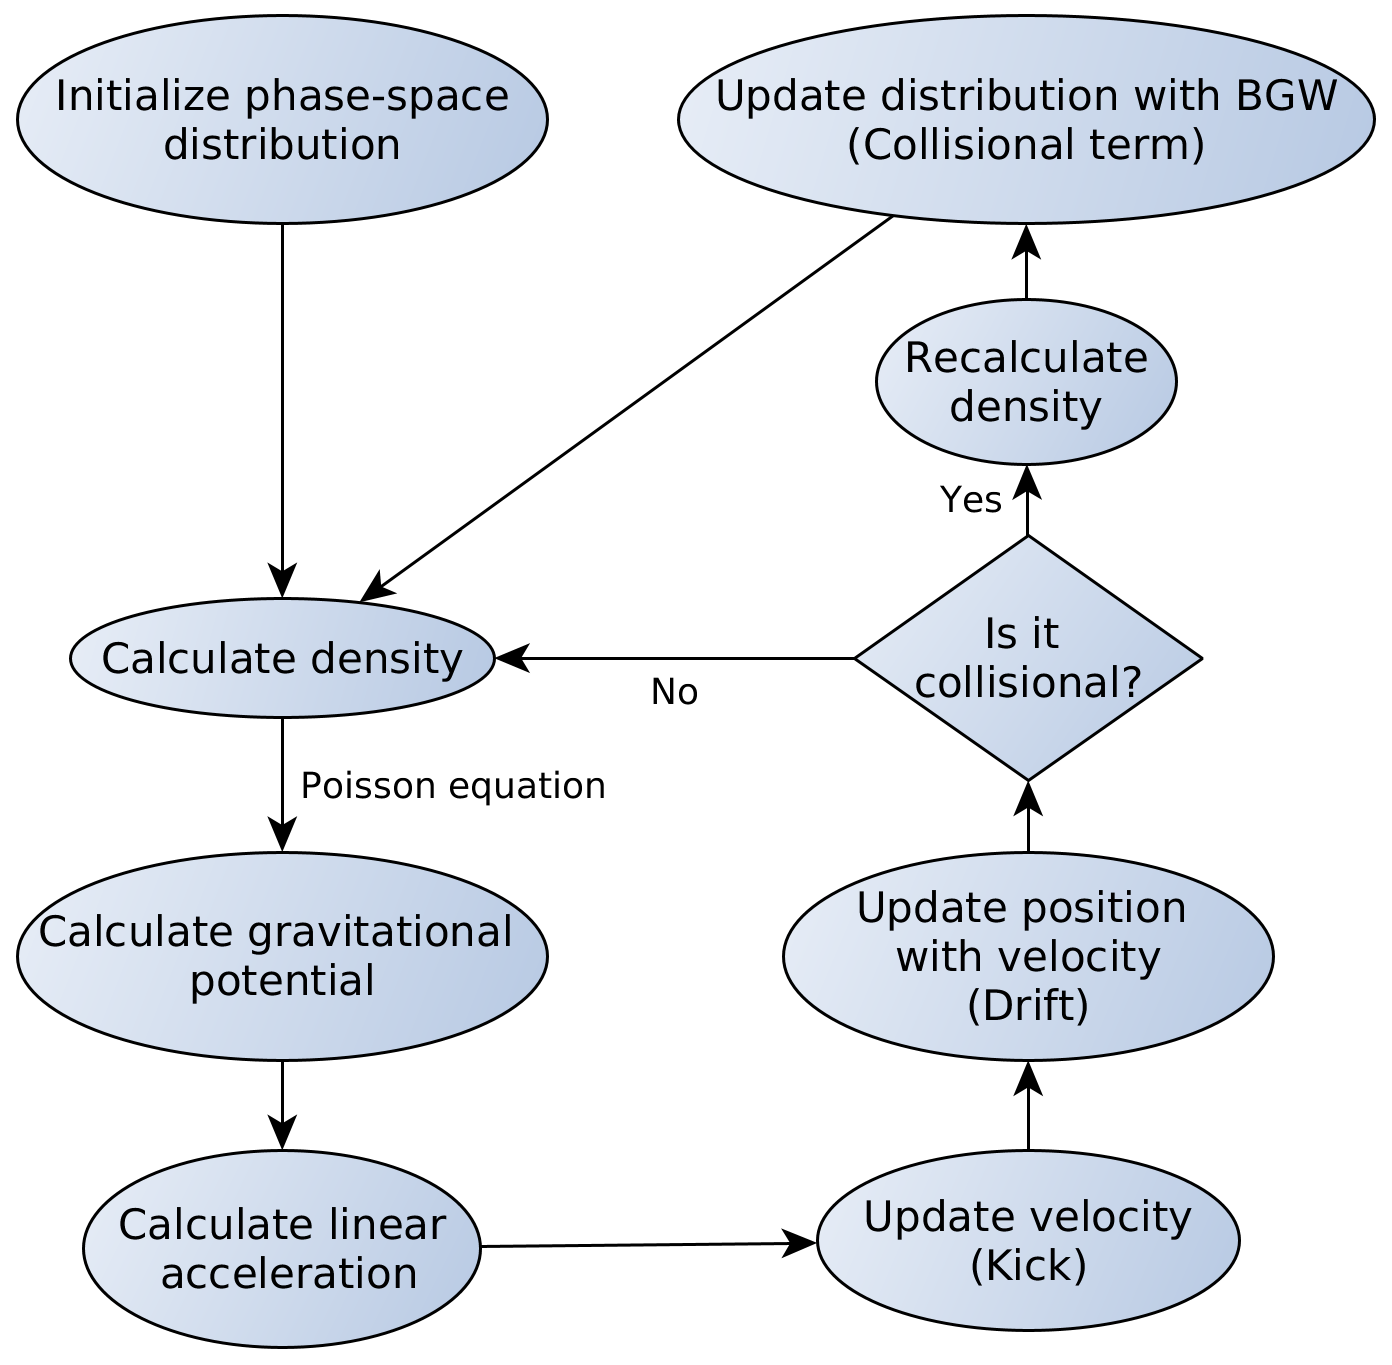
\includegraphics[scale=0.2]{imag/flowchart.png}
    \caption{Flowchat of the algorithm.}
    \label{flowchart}
\end{figure}



Given the density-velocity phase space, the spatial density of matter is given by the integral: $$ \dens[t] = \int_{-\infty}^{\infty} \! \f[t] \, \dd \vb{v}. $$ Which, when evaluating in the lattice becomes:
\begin{equation}
\dens[t] = \sum_{\vb{V}_{min}}^{\vb{V}_{max}} \f[t] \, \dd \vb{v}
\end{equation}
and during initialization:
\begin{equation}
\dens[0] = \sum_{\vb{V}_{min}}^{\vb{V}_{max}} \f[0] \, \dd \vb{v}
\end{equation}

Once we have calculated the density, we can use the Poisson equation to calculate the potential due the gravitational force\cite{integerLatticeDynamics}

\begin{equation}
\laplacian \pot = 4 \pi G \dens
\end{equation}

To solve the Poisson equation we use the pseudo-spectral Fourier method, which allows for very fast numerical solutions by making use of the Fast Fourier Transform algorithm. The idea is simply to apply a Fast Fourier Transform (FFT), then solve the equation in the Fourier space, and then apply an inverse transform (IFFT). In the phase space the Poisson equation is given by\cite{freePoisson} \cite{computerUsingParticles}

\begin{equation}
\lambda_{\vb{k}}^2 \hat{\Phi}(\vb{k},t) = 4 \pi G \hat{\rho}(\vb{k},t)
\end{equation}

Where $\hat{g}(\vb{k},t)$ is the Fourier transform of $g(\vb{r},t)$, and $\lambda_{\vb{k}}$ is a constant that depends on the size of the lattice and the wavevector $\vb{k}$. $\lambda_{\vb{k}}$ is calculated according to the approximation scheme used to solve the equation, here we use the pseudo-spectral approximation, in which $\lambda_{\vb{k}}$ becomes:

\begin{equation}
\lambda_{\vb{k}}^2 = \qty(\frac{2 \pi k_x}{X_{max} - X_{min}})^2 + \qty(\frac{2 \pi k_y}{Y_{max} - Y_{min}})^2 + \qty(\frac{2 \pi k_z}{Z_{max} - Z_{min}})^2
\end{equation}

Therefore, solving the Poisson equation is reduced to calculating $\hat{\Phi}(\vb{k})$ for every $\vb{k}$ and then transforming out of Fourier space.

Once we have the potential, calculating the acceleration is straight-forward:
\begin{equation}
\acce = -\grad \pot
\end{equation}
Which, in the context of the lattice can be calculated simply with a central difference numerical derivative.
Now, in order to update the phase space, we must first define the time interval to simulate: we name $N_t$ the number of time intervals to simulate and $\dd t$ the length of each of such intervals.
After calculating the acceleration and defining $\dd t$, we can update our phase space, the subtlety here is that we will only use integer arithmetic, which means that we do not exactly care for the change in velocity during a time $\dd t$ but for how many cells in the phase space that change represents. This is modeled by:
\begin{equation}
\vb{v}_{n+1} = \vb{v}_n + \toInt{\vb{a}_n \dd t}
\end{equation}
With $\toInt{x}$ representing the operator \tqt{to nearest integer}, so that $\vb{v}$ and $\toInt{\vb{a} \dd t}$ are vectors of integers and $n$ represents the time instant. The update of the velocity is known as \tqt{kick}. Analogously, the update of the position is known as \tqt{drift}, and is given by:
\begin{equation}
\vb{r}_{n+1} = \vb{r}_n + \toInt{\vb{v}_n \dd t}
\end{equation}

Using only integer arithmetics allows for the elimination of the rounding error but introduces lattice noise. Regardless, this method creates a one to one map with the continous solution.\cite{franco} \cite{integerLatticeDynamics}

The \tqt{kick} and \tqt{drift} together are known as the \tqt{Streaming} step, and it represents the classical movement of particles under a potential but without considering the collision of particles. If we want a collisionless simulation, we can just calculate again the density and continue the algorithm from there. If we want a collisional simulation, we must define a collisional step.

\section{The Collisional Step}
As previously mentioned, solving the collisional integral $C[f]$ is not straight-forward, as it depends on the modeling of the short range interactions between particles that we decide to assign to the dark matter particle. Given that the short range interaction of dark matter is uncertain, we avoid using an specific description of the microscopic interaction and choose to use a mesoscopic approach, as discussed in section \ref{bgk}. The BGK collisional operator is given by:\\
\begin{equation}
C[f] = -\frac{1}{\tau}(\f - f_e(\rv))
\end{equation}

\section{Units and Systems to Simulate}




















\chapter{Results}
\section{No Collisional}
\section{Collisional with reported $<\sigma v>$}
\section{Different Equlibrium Distributions}